\section{Basic Antenna Parameters}
\label{sec:basicantennaparams}
\begin{aautop}
This section will give a summery of the fundamental theories and parameters that are used to describe antennas. This should give a basic understanding of antennas. The parameters described in this section are used throughout the report. 
\end{aautop}

\subsection{Antenna Definition}
\label{subsec:antenna-def}
The IEEE defines an antenna as ``a means for radiating or receiving radio waves''. In other words, the purpose of an antenna is to make the transition from a signal in a transmission line to electromagnetic fields in the air. An antenna will radiates an electric field (E-field) in a given direction, which then induces a magnetic field (H-field) orthogonal to the E-field. This relation is described by Maxwell's Equations which is covered in Section~\ref{sec:fdtd} \cite{balanis2012antenna}.

\subsection{Isotropic Radiator}
\label{subsec:isotropic-ant}
An isotropic antenna, can be represented as a point source. The isotropic antenna radiates its power uniformly in a sphere. The power density, $S_{\text{iso}}$, can be expressed as the source power $P_s$ over the surface area of a sphere which is given by $4\pi r^2$ \cite{balanis2012antenna}:
\begin{align} %% 
    S_{\text{iso}} = \frac{P_s}{4\pi r^2}
\end{align}
Clearly, it is not possible to construct such an antenna. However, this is used as a reference for quantifying other properties of an antenna. These properties could be the gain or directivity (see Section \ref{subsec:dir_gain}), and the unit would then be in \si{dBi} rather than \si{dB}.

\subsection{Radiation Pattern}
\label{subsec:radiation-p}
The radiation pattern describes how the antenna emits or receives radiated power. This is commonly visualized by a 3D plot or 2D cuts of the 3D plot in specific coordinates. The unit of power used is often gain or directivity (see Section~\ref{subsec:dir_gain}) and this is often compared to the isotropic antenna \cite{balanis2012antenna}.

\subsection{Field Regions}
The waves transmitted from the antenna are usually grouped into three regions of radiation, based on how the waves propagate and the field structure \cite{balanis2012antenna}. Obviously, there is no abrupt change, but rather a continuous change.
\begin{itemize}
\item The Reactive near-field.
\item The Radiating near-field (Fresnel).
\item The Farfield.
\end{itemize}

The reactive near-field is defined as the portion of the near-field region immediately surrounding the antenna wherein the reactive field predominates \cite{balanis2012antenna}. The outer boundary for this region is given by \cite{balanis2012antenna}
\begin{align} %%
  R < 0.62 \sqrt{D^3/\lambda}
\end{align}
where $D$ is the largest dimension of the antenna. To be valid, $D$ must also be large compared to the wavelength.

The radiating near-field is defined as the region between the reactive near-field and the far-field. This field may not exist in the case that the overall antenna dimension is very small compared to the wavelength. The outer boundary for this is defined as \cite{balanis2012antenna}
\begin{align} %%
  R \leq 2D^2/\lambda
\end{align}

The far-field region is defined as the region of the field where the angular field distribution is independent of the distance, that is the radiation pattern does not change shape with distance. The far-field is also dominated by fields where the E- and H-fields are orthogonal and propagates as plane waves. The inner boundary is given as \cite{balanis2012antenna}
\begin{align} %%
  R > 2D^2/\lambda
\end{align}
The three different regions are illustrated on Figure~\ref{fig:field-regions}. 

\begin{figure}[htbp]
  \centering
  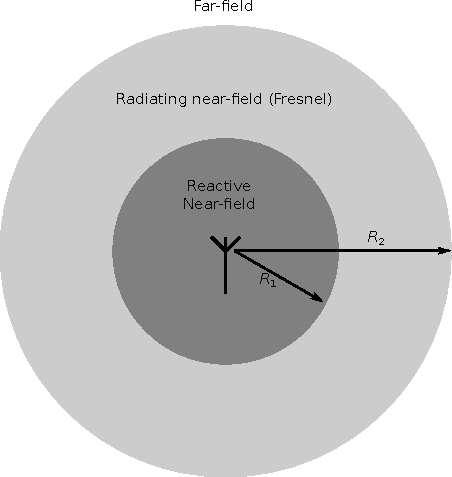
\includegraphics[scale=1]{img/analysis/radiationfields}
  \caption{Visualization of different fields \cite{balanis2012antenna}.}
  \label{fig:field-regions}
\end{figure}

\subsection{Directivity and Gain}
\label{subsec:dir_gain}
Directivity is defined as the ratio of the power radiated at a point with a certain angle and distance from the antenna compared to what would be radiated from a reference isotropic antenna. Mathematically, it can be written as \cite{balanis2012antenna}
\begin{align} %%
  D = \frac{U}{U_0} = \frac{4 \pi U}{P_{rad}} 
\end{align}
where
\begin{where}
  \item[$D$] Directivity.
  \item[$U$] Radiation intensity.
  \item[$U_0$] Radiation intensity of an isotropic source.
  \item[$P_{rad}$] Total radiated power.
\end{where}
It should be noted, that for this equation to be valid, the waves must propagate as plane waves, thus being in the farfield region.

Gain is a measure closely related to directivity. It takes the efficiency of the antenna into account as well as the direction. The gain is defined as the ratio of the intensity in a given direction to the radiant intensity that would be obtained if it was radiated isotropically. In mathematical form, it can be expressed as \cite{balanis2012antenna}:
\begin{align} %%
  G = 4 \pi \frac{\text{radiation intensity}}{\text{total accepted input power}} = 4 \pi \frac{U(\theta,\phi)}{P_{\text{in}}}
\end{align}
In many cases, the relative gain is used, which is defined as the ratio of the power gain in a given direction to the power gain of a reference antenna in its referenced direction. The reference antenna could be a dipole, horn, etc. 

The gain can also be calculated using the directivity, since they are only related by the efficiency. This is given as \cite{balanis2012antenna}
\begin{align} %%
  G(\theta,\phi) = \eta_{cd}D(\theta, \phi)
\end{align}

\subsection{Impedance, Return Loss, and VSWR}
The impedance and matching is an important part of the antenna design to ensure maximum power transfer. The input impedance of an antenna is defined as $Z_{\text{in}}$. From the classical circuit theory it is known that the maximum power transfer occurs when the in- and output impedance is matched (see Section~\ref{sec:tuners}). If there is a mismatch, some of the power will be reflected back into the source, and thus not transmitted from the antenna. The reflection coefficient $\Gamma$ is defined as \cite{pozar2011microwave}
\begin{align}%%
    \Gamma = \frac{Z_{\text{in}}-Z_0}{Z_{\text{in}}+Z_0}
\end{align}
where
\begin{where}
\item[$Z_0$] The characteristic impedance, which is typically \SI{50}{\ohm}.
\end{where}
The reflection coefficient is often expressed in \si{dB}. 

Another closely related figure is the Voltage Standing Wave Ratio (VSWR), and is defined as \cite{pozar2011microwave}
\begin{align}%%
  \text{VSWR} = \frac{1+|\Gamma|}{1-|\Gamma|} 
\end{align}

\subsection{Bandwidth}
The bandwidth of an antenna defines the usable spectrum of the antenna. The required bandwidth is dependent on the modulation schemes used, which makes the bandwidth an important part of the antenna design. The bandwidth is typically defined with respect to a given reflection coefficient or VSWR, e.g.\ at a reflection coefficient of 0.25 (or \SI{-6}{dB}).

\subsection{Polarization}
The polarization in a certain direction is simply defined as the polarization of the transmitted wave by the antenna. It describes the time-varying direction at a relative magnitude of the E-field vector analogously to the polarization of light. Polarization can be classified into groups such as linear, circular, or elliptical polarization. If a transmit antenna and a receive antenna are of different polarization, this will introduce a polarization mismatch loss to the system \cite{balanis2012antenna}.

\subsection{Antenna Efficiency}
There are a lot of different measures for antenna efficiency depending on which losses that are taken into account. The total efficiency takes the losses from the input terminal and within the antenna structure into account \cite{balanis2012antenna}. This can in general be expressed as \cite{balanis2012antenna}
\begin{align}%%
\label{eq:ant-eff}
  \eta_0 = \eta_r \eta_c \eta_d 
\end{align}
where
\begin{where}
\item[$\eta_0$] Total efficiency.
\item[$\eta_r$] Mismatch loss.
\item[$\eta_c$] Conduction efficiency.
\item[$\eta_d$] Dielectric loss.
\end{where}
The conduction and dielectric losses are hard to compute, and by measurements they cannot be separated \cite{balanis2012antenna}.

\subsubsection{Radiation Efficiency}
The radiation efficiency is defined as the conduction-dielectric efficiency $\eta_r = \eta_{cd}$ which is defined as the ratio of the power delivered to the radiation resistance, $R_r$, to the power delivered to $R_r$ and $R_L$ (loss) in total \cite{balanis2012antenna}. This can be written as \cite{balanis2012antenna}
\begin{align} %%
  \eta_r = \frac{P_{\text{radiated}}}{P_{\text{input}}} = \frac{R_r}{R_L+R_r}
\end{align}

\subsection{Antenna $Q$-Factor}
As it will be described in Section~\ref{sec:elsmallantennas}, the size of an antenna sets the lowest achievable Quality Factor (or $Q$-factor) of an antenna. In this section, the relation between $Q$-factor and antenna bandwidth will be described as well as the impact of having multiple antennas on the $Q$-factor.

The $Q$-factor is a measure of loss in a resonant circuit \cite{pozar2011microwave}. A higher $Q$ means lower loss. In an antenna, it is desired to have loss due to radiation while mismatch loss, conductive loss, and dielectric loss is undesirable. The $Q$ due to radiation should therefore be low to get a high degree of radiation.

\begin{figure}[htbp]
    \centering
    \begin{subfigure}[t]{0.49\linewidth}
        \centering
        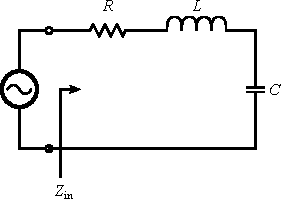
\includegraphics{img/analysis/q_series}
        \caption{Series.}
    \end{subfigure}
    \hfill
    \begin{subfigure}[t]{0.49\linewidth}
        \centering
        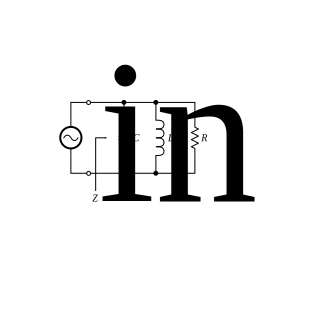
\includegraphics{img/analysis/q_shunt}
        \caption{Parallel.}
    \end{subfigure}
    \caption{Series and parallel resonant circuit equivalent of a single-resonance antenna.}
    \label{fig:qresonanteq}
\end{figure}

For a single-resonance antenna, a resonant circuit can often be used as an equivalent for the antenna. A series and a parallel equivalent circuit is shown in Figure~\ref{fig:qresonanteq}. A circuit is at resonance when the reactive part, $X_0=0$. For an antenna, it is desired to have a resonance where $R_0$ is equal to the characteristic impedance of the system (e.g.\ \SI{50}{\ohm}). For a multi-resonance antenna, a resonant circuit equivalent can be used for each resonance, given that the bandwidth of observation is chosen narrow enough (by altering the $\beta$-parameter below) \cite{yaghjian2005impedance}.
% Resonace = X0 = 0
% Multi-resonance: Locally, resonant circuits

An investigation of the relation between impedance, bandwidth, and $Q$ of antennas by Yaghjian and Best \cite{yaghjian2005impedance}. They developed the following exact expression for the $Q$-factor:
\begin{equation}%%
    Q(\omega_0) = \left| 
    \frac{\omega_0}{2R_0(\omega_0)}X_0^{\prime}(\omega_0)
    -
    \frac{2\omega_0}{|I_0|^2 R_0(\omega_0)} [W_L(\omega_0) + W_R(\omega_0)]
    \right|
\end{equation}
where
\begin{where}
\item[$\omega_0$] Radian frequency at which the antenna is tuned.
\item[$R_0(\omega_0)$] Input resistance at resonance.
\item[$X^{\prime}_0(\omega_0)$] Derivative of the input reactance with respect to $\omega$, evaluated at $\omega_0$.
\item[$I_0$] Current fed to the antenna.
\item[$W_L$] Energy associated with power loss in the antenna, computed from the electric and magnetic fields.
\item[$W_R$] Energy associated with the power radiated by the antenna, computed from the farfield.
\end{where}
In the same paper, an approximate expression is developed for the $Q$-factor based on the input impedance at resonance. Furthermore, an approximation is developed based on the fractional bandwidth, $\text{FBW}_V$:
\begin{align}%%
    Q(\omega_0) 
    \label{eq:qapprox1}
    &\approx \frac{\omega_0}{2R_0(\omega_0)} |Z_0^{\prime}(\omega_0)| \\
    \label{eq:qapprox2}
    &\approx \frac{2\sqrt{\beta}}{\text{FBW}_V(\omega_0)}, & \sqrt{\beta} = \frac{s-1}{2\sqrt{s}} \leq 1
\end{align}
where $s$ is the requirement VSWR at which the bandwidth is determined. The approximation is based on the assumption that $W_L$ and $W_R$ are ohmic losses in the resonance equivalent circuits \cite{yaghjian2005impedance}. Furthermore, the derivatives, $R^{\prime}_0(\omega)$ and $X^{\prime}_0(\omega)$ must not change greatly over the bandwidth of the antenna -- which holds by choosing the bandwidth narrow enough \cite{yaghjian2005impedance}.
Finally, is is assumed that the antenna is linear (i.e.\ there is a linear relationship from the $\mathbf{B}$ and $\mathbf{D}$ fields to the $\mathbf{H}$ and $\mathbf{E}$ fields), passive (non-gain media), and tuned by only passive circuitry \cite{yaghjian2005impedance}. 

The approximation in Equation~\ref{eq:qapprox1} can be used to compute the $Q$ of an antenna by knowing its input impedance. This relation explains how the $Q$ may be affected by having multiple antennas by taking into account the mutual impedance between the antennas \cite{balanis2012antenna}.

The approximation in Equation~\ref{eq:qapprox2} is useful for approximating the bandwidth of an antenna based on a $Q$-factor. This $Q$ could, for example, be computed using the Chu limit (see Section~\ref{sec:fun_lim}) and thus, the highest possible bandwidth of an antenna of a given size could be computed. Alternatively, the formula could be used to approximate the $Q$ of an antenna with a given resonance by rearranging the equation.

\FloatBarrier
\subsection{Mobile Antenna Limitations}
\label{subsec:ant_limit}
As the requirements for mobile antennas get more and more strict, some trade off's need to be considered when designing an antenna.
The design constrains when designing antennas is a trade off between size, bandwidth, and efficiency, as illustrated in Figure \ref{fig:antenna_tradeoff}. 
The trade off relationship can be expressed as \cite{hilbert2015tradeoff}
\begin{align} %%
  \frac{\Delta f}{f} \propto \frac{(a/ \lambda)^3}{\eta}
\end{align}
where
\begin{where}
\item [$\lambda$] Wavelength.
\item [$\eta$] Efficiency.
\item [$\Delta f / f$] Bandwidth.
\item [$a^3$] Antenna volume.
\end{where}
This relationship describes that it is hard to design a small antenna with excellent efficiency performance and a high bandwidth.
Therefore, when designing mobile antennas that requires high bandwidth and small antenna structures, a trade-off is needed to ensure that the antenna performs as required \cite{hilbert2015tradeoff}.

In the case of this project, the antenna is required to have a bandwidth from \SI{700}{MHz} to \SI{960}{MHz} in the low band and from \SI{1710}{MHz} to \SI{2650}{MHz} in the high band. Furthermore, it needs to be very small with a maximum ground clearance of \SI{10}{mm} and an efficiency above \SI{50}{\percent} in the entire bandwidth. Due to the constraints on the antenna size when designed for mobile phones, the bandwidth and efficiency will be limited. This leads to design challenges in exploiting the available and limited volume within a sphere \cite{balanis2012antenna}.
As it is hard to get both high efficiency and high bandwidth with a small fixed-tuned antenna, a frequency reconfigurable antenna system could be one way of covering a high bandwidth with a small antenna \cite{hilbert2015tradeoff}.  

\begin{figure}[htbp]
    \centering
  % 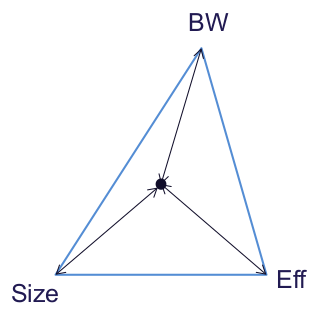
\includegraphics[scale=0.4]{img/analysis/antenna_limitations}
    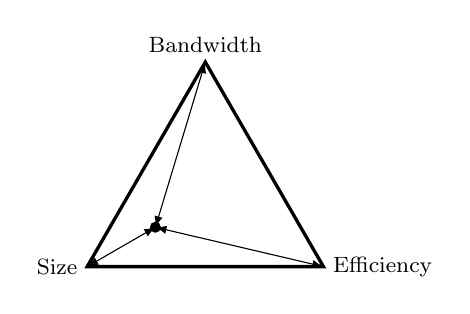
\begin{tikzpicture}[>=latex, font=\footnotesize]
        \draw [very thick] (0,0) coordinate(a) -- ++(60:3) coordinate(b) -- ++(-60:3) coordinate(c) -- cycle;
        \node [left] at (a) {Size};
        \node [above] at (b) {Bandwidth};
        \node [right] at (c) {Efficiency};

        \path[fill=black] (30:1) coordinate(p) circle (2pt);
        \draw[<->] (a) -- (p);
        \draw[<->] (b) -- (p);
        \draw[<->] (c) -- (p);
    \end{tikzpicture}
    \caption{Antenna design trade-off's.}
    \label{fig:antenna_tradeoff}
\end{figure}

\FloatBarrier
\subsection{Internal Antennas}
As described in the antenna limitation section, Section~\ref{subsec:ant_limit}, the size restriction of mobile phone antennas limits the bandwidth and efficiency.
These are only a few of the affected parameters considered when dealing with internal antennas. Going from external to internal antenna designs influences the radiation pattern, matching, and impedance bandwidth. The losses and detuning caused by the user can also have a higher influence, as the hand of the user generally moves closer to the antenna structure compared to the external antenna case \cite{fujimoto2008mobile}. 

The internal antenna design is also deeper affected by the chassis and PCB size \cite{sanchez2008multiband}. An example of the influence of the PCB size on the resonant frequency and the bandwidth can be seen in Figure~\ref{fig:antenna_pcb_behavior}. The example is done with a $\SI{40}{mm} \times l\,\si{mm}$ dual-band patch antenna over a metallic ground plane for the frequencies \SI{900}{MHz} in the GSM band and \SI{1975}{MHz} in the DCS band. The exact frequencies used in the simulation is the center frequency of each band. 

As seen in the Figure \ref{fig:antenna_pcb_behavior}, both the resonant frequency and the bandwidth is greatly affected by the size of the ground plane -- especially the GSM band at \SI{900}{MHz}. When the ground plane and the antenna both are in resonance state, the maximum bandwidth is achieved. In the case of MIMO antenna designs with two antennas, one on the bottom and one of the side of the PCB, the maximum bandwidth is hard to achieve with two identical antenna designs \cite{sanchez2008multiband}. 

\begin{figure}[htbp]
   \begin{subfigure}[b]{0.49\linewidth}
        \centering
        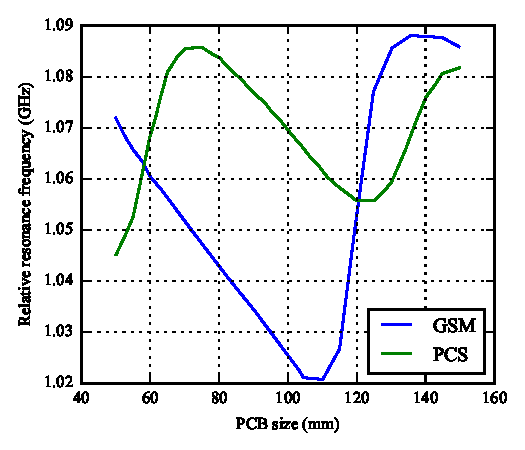
\includegraphics{img/analysis/pcbsize_freq.pdf}
        \caption{Ground plane size effect on the resonance frequency.}
    \end{subfigure}
    \hfill
    \begin{subfigure}[b]{0.49\linewidth}
        \centering
        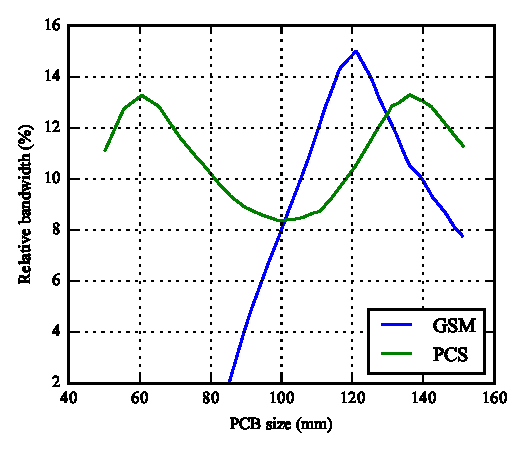
\includegraphics{img/analysis/pcbsize_bandwidth.pdf}
        \caption{Ground plane size effect on the bandwidth at \SI{-6}{dB}.}
    \end{subfigure}
    \caption{Ground plane size effect on the resonance frequency and the bandwidth\cite{sanchez2008multiband}.}
    \label{fig:antenna_pcb_behavior}
\end{figure}

For internal antennas, the small size, high efficiency, and high bandwidth are only a few of the design requirements. The design requirements also include \cite{fujimoto2008mobile}:
\begin{itemize}
\item Light weight.
\item Compactness.
\item Low profile.
\item Robustness.
\item Flexibility.
\item Integration with nearby materials.
\end{itemize}
Most of these requirements and factors needs to be considered in the design and choosing of the antenna type. Robustness comes with the fact that it is an internal antenna and therefore is protected by the phone case. Some of the most used antenna types for mobile antennas are the PIFA and the folded monopole antennas. Both designs are suitable for mobile phones, as the antenna size is a $1/4 \lambda$ \cite{fujimoto2008mobile}.

As mentioned, the PCB has a big influence on the antenna, but the antenna performance is also degraded by other components such as the display, camera, flex-films, speaker, microphone, etc. When activated, these digital components work at high speed and will degrade the receiving sensitivity and cause problems to the receiving bands, as the components emits RF noise. When the components are deactivated, the components will work as passive lossy loading elements. Close to the antenna, the passive components will cause reduction to the effective antenna volume, detuning, and ohmic losses \cite{fujimoto2008mobile}.

Because of the large battery size in today's smartphones, the battery can have a significant impact on the antenna performance. If placed closely to the antenna, the battery can introduce an induced current on the antenna and affect the performance. To have as little impact as possible from the battery it should be placed at a distance of \SIrange{4}{6}{mm} or more from the antenna \cite{fujimoto2008mobile}. 

The display is parallel to the PCB ground plane and is made of lossy dielectric material, which can change the EM near field of the antenna. In most phones, the display is large and can have a big influence on the antenna performance, as the display introduces some induced currents on the antenna \cite{fujimoto2008mobile}.   

\subsection{Electrically Small Antennas}
\label{sec:elsmallantennas}
The concept and definition of electrically small antennas was introduced by Wheeler in 1947 \cite{wheeler1947}, and is given by
\begin{align} %%
\label{eq:esa-def}
  ka \ll 1
\end{align}
where 
\begin{where}
\item[$k$] $2\pi / \lambda$ is the wave number. 
\item[$a$] The radius of a sphere enclosing the maximum dimension of the antenna. 
\end{where}
The parameter $a$ is illustrated in Figure~\ref{fig:ant-esa-def}. Inserting the definition of $k$ yields that
\begin{align} %%
  \frac{2\pi a}{\lambda} \ll 1
\end{align}
in order for an antenna to be defined as electrically small. It should also be noted that if the antenna is used with a small ground plane, which often is the case, then the ground plane itself becomes a dominant part of the antenna structure. In this case, the entire ground plane must be included in the sphere and thus in the definition of $a$.

\begin{figure}[htbp]
  \centering
  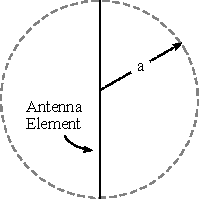
\includegraphics[scale=1]{img/analysis/ESA}
  \caption{Illustration of ESA definition.}
  \label{fig:ant-esa-def}
\end{figure}

\subsubsection{Fundamental Limits of Q}
\label{sec:fun_lim}
L.\ J.\ Chu quantified the relationship between the minimum $Q$ of an electrically small antenna and the physical size relative to the wavelength \cite{chu1948}. This relationship was later corrected by McLean \cite{mclean1996} to be
\begin{align} %%
  Q_L = \frac{1}{k^3a^3}+ \frac{1}{ka}
\end{align}
for a linear antenna in free space.

\subsection{Friis Transmission Equation}
The Friis transmission equation relates the power received with the power transmitted. In the most simple form, the Friis transmission equation is based on the free-space path loss (FSPL), the gains of the antennas, and the transmit power. The free-space path loss (or ``path gain'' as this notation is a decaying with distance) is defined as \cite{balanis2012antenna}
\begin{align} %%
  \label{eq:fspl}
  \text{FSPL} = \left( \frac{\lambda}{4 \pi d} \right)^2 
\end{align}
where
\begin{where}
\item[$\lambda$] Wavelength.
\item[$d$] Distance from the transmitter to the receiver.
\end{where}
This assumes that the energy spreads out in a sphere and that the only loss is from the distance. It is seen that the power decreases with the square of the range, which is plotted in Figure~\ref{fig:fspl-plot} for a \SI{2.6}{GHz} link.

\begin{figure}[htbp]
  \centering
  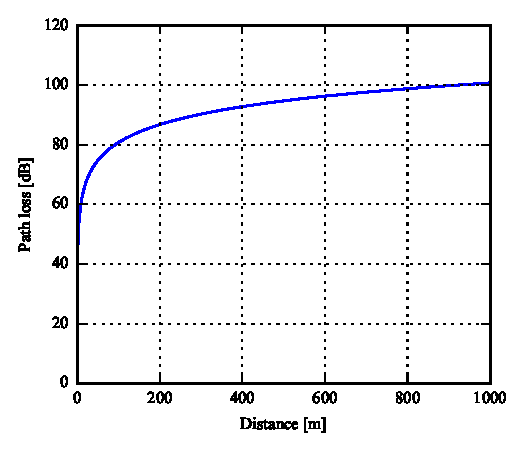
\includegraphics{img/analysis/distancePathloss}
  \caption{Free space path loss in dB for a \SI{2.6}{GHz} link.}
  \label{fig:fspl-plot}
\end{figure}

The Friis Transmission equation in its most basic form can be written as \cite{balanis2012antenna} 
\begin{align}%%
    \frac{P_r}{P_t} = \left( \frac{\lambda}{4 \pi d} \right)^2 G_{t} G_{r} 
\end{align}
where
\begin{where} 
\item[$P_r$] Power received.
\item[$P_t$] Power transmitted.
\item[$G$] Transmitter and receiver gains.
\end{where}
In this case, it is assumed that there is no impedance or polarization mismatch. It is also assumed that the two antennas are aligned perfectly. Finally, it is assumed that the path loss is described by FSPL, which in reality is a very rare case. The next section will describe a few more realistic propagation models.


\begin{aautail}
Throughout this section the basic antenna parameters have been described. In the next section, the effect of matching circuitry and tuners will be described.
\end{aautail}
